\documentclass[10pt]{article}
\usepackage[ruled, linesnumbered]{algorithm2e}
\usepackage{Jan1, epsfig, subfigure, amssymb, multirow, algorithmic,amsmath}
\usepackage{latexsym,amssymb,epsfig,graphicx,subfigure,rotating,multirow,colortbl,xcolor,amsmath,algorithmic,booktabs,url}
\usepackage{accents}

\textwidth 160mm
\textheight 225mm
\voffset 1mm
\oddsidemargin 1mm
\evensidemargin 1mm
\newtheorem{definition}{Definition}
\newtheorem{theorem}{Theorem}
\newtheorem{proposition}{Proposition}
\newtheorem{conjecture}{Conjecture}
\newtheorem{corollary}{Corollary}
\newtheorem{lemma}{Lemma}
\newtheorem{example}{Example}


\usepackage[english]{babel}
\usepackage{blindtext}

\usepackage{lipsum}

\newcommand\blfootnote[1]{%
  \begingroup
  \renewcommand\thefootnote{}\footnote{#1}%
  \addtocounter{footnote}{-1}%
  \endgroup
}






\title{ \hspace{3.2cm}
\includegraphics[scale=0.3]{./Fig/1.png} \newline \newline \newline  \LARGE{Comparison of QSS Solver's LIQSS2 solver with OpenModelica's DASSL solver}}

% \author{\large{Comparison of QSS Solver's LIQSS2 solver} \large{with OpenModelica's DASSL solver}}

% \date{\HUGE{Comparison of QSS Solver's LIQSS2 solver} \large{with OpenModelica's DASSL solver}}
\date{}


\renewcommand{\thefigure}{\arabic{section}.\arabic{figure}}
\renewcommand{\thetable}{\arabic{section}.\arabic{table}}
\begin{document}
\setcounter{page}{1}



\newcommand{\blokkie}{\hspace{.07cm}\Box\hspace{.07cm}}

%%%%% Set up the coloured tables %%%%%
\colorlet{tableheadcolor}{gray!25} % Table header colour = 25% gray
\colorlet{tablerowcolor}{gray!10} % Table row separator colour = 10% gray
\newcommand{\headcol}{\rowcolor{tableheadcolor}}
\newcommand{\rowcol}{\rowcolor{tablerowcolor}}

% The top-most line of a table
\newcommand{\topline}{\arrayrulecolor{black}\specialrule{0.1em}{\abovetopsep}{0pt}%
	\arrayrulecolor{tableheadcolor}\specialrule{\belowrulesep}{0pt}{0pt}%
	\arrayrulecolor{black}}

	% The top-most line of a table
\newcommand{\toplinee}{\arrayrulecolor{black}\specialrule{0.1em}{\abovetopsep}{0pt}%
	\arrayrulecolor{tablerowcolor}\specialrule{\belowrulesep}{0pt}{0pt}%
	\arrayrulecolor{black}}

% The line between the headings and the table body
\newcommand{\midline}{\arrayrulecolor{tableheadcolor}\specialrule{\aboverulesep}{0pt}{0pt}%
	\arrayrulecolor{black}\specialrule{\lightrulewidth}{0pt}{0pt}%
	\arrayrulecolor{white}\specialrule{\belowrulesep}{0pt}{0pt}%
	\arrayrulecolor{black}}

% A line for when the upper row is rowcolor and the next line is white
\newcommand{\midlinecbw}{\arrayrulecolor{tablerowcolor}\specialrule{\aboverulesep}{0pt}{0pt}%
	\arrayrulecolor{black}\specialrule{\lightrulewidth}{0pt}{0pt}%
 	\arrayrulecolor{white}\specialrule{\belowrulesep}{0pt}{0pt}%
	\arrayrulecolor{black}}

% A line with no black, to further separate a rowcolor row and a white row
\newcommand{\midlinecw}{\arrayrulecolor{tablerowcolor}\specialrule{\aboverulesep}{0pt}{0pt}%
	\arrayrulecolor{tablerowcolor}\specialrule{\lightrulewidth}{0pt}{0pt}%
	\arrayrulecolor{white}\specialrule{\belowrulesep}{0pt}{0pt}%
	\arrayrulecolor{black}}

% A line for when the upper row is white and the next line is rowcolor
\newcommand{\midlinewbc}{\arrayrulecolor{white}\specialrule{\aboverulesep}{0pt}{0pt}%
	\arrayrulecolor{black}\specialrule{\lightrulewidth}{0pt}{0pt}%
	\arrayrulecolor{tablerowcolor}\specialrule{\belowrulesep}{0pt}{0pt}%
	\arrayrulecolor{black}}

% sadfsdfsdf sdfsdfsdf
\newcommand{\midlinehr}{\arrayrulecolor{tablerowcolor}\specialrule{\aboverulesep}{0pt}{0pt}%
	\arrayrulecolor{black}\specialrule{\lightrulewidth}{0pt}{0pt}%
	\arrayrulecolor{tableheadcolor}\specialrule{\belowrulesep}{0pt}{0pt}%
	\arrayrulecolor{tablerowcolor}}


% A line for the bottom of the table, when the last row is white
\newcommand{\bottomline}{\arrayrulecolor{white}\specialrule{\aboverulesep}{0pt}{0pt}%
	\arrayrulecolor{black}\specialrule{\heavyrulewidth}{0pt}{\belowbottomsep}}%

% A line for the bottom of the table, when the last row is rowcolor
\newcommand{\bottomlinec}{\arrayrulecolor{tablerowcolor}\specialrule{\aboverulesep}{0pt}{0pt}%
	\arrayrulecolor{black}\specialrule{\heavyrulewidth}{0pt}{\belowbottomsep}}%

\newcommand{\bottomlinect}{\arrayrulecolor{tableheadcolor}\specialrule{\aboverulesep}{0pt}{0pt}%
	\arrayrulecolor{black}\specialrule{\heavyrulewidth}{0pt}{\belowbottomsep}}%
%%%%% Set up the coloured tables %%%%%



\maketitle



\pagestyle{myheadings}


\section{Introduction}

\blfootnote{Subject to NDA: Confidential \& Proprietary \copyright\ 2016 by LifeQ Global Limited. All Rights Reserved.}

This document contains a detailed comparison of LifeQ's LIQSS2 solver (which is programmed within the OpenModelica framework) and OpenModelica's DASSL solver. The actual results and the simulation times are of importance. A number of models will be simulated for various tolerances and simulation times in order to gain insight into the quality of the solvers.


\section{The solvers}

All the solvers used have been mentioned in \S1 of this document. These solvers include:
\begin{itemize}
 \item OpenModelica DASSL ({\sf DASSL})
 \item LifeQ's LIQSS2 solver ({\sf LIQSS2})
\end{itemize}

\section{Simulation details}

For each simulation run, the following will be specified:
\begin{itemize}
 \item duration of the simulation,
 \item some key state variables that will be investigated,
 \item the actual completion time of the simulation, and
 \item a conclusion of the obtained results.
\end{itemize}

For the DASSL solver in OpenModelica the number of intervals will be fixed at $10\,000$ for all simulations.

The tolerances for both solvers will be varied for the various model being simulated. The LifeQ LIQSS2 solver has two tolerances --- a {\em relative tolerance} as well as an {\em absolute tolerance}. The absolute tolerance will be set at 0.001 times the absolute tolerance throughout all the simulations in this document.

An Intel(R) Core(TM) i7-4710MQ CPU @ 2.50GHz computer containing 8 processors and 16GB RAM,
using operating system Linux Ubuntu 16.04 was used for the tests.



\section{Results}

The numerical results and related finding will be considered in this section. The computational times reported are in seconds and are the sum of the {\tt{user}} time and {\tt{sys}} time provided by the UNIX {\tt{time}} command, which is used in conjunction with the executable that is built for each model. The {\tt{user}} time is defined as the {\em total number of CPU-seconds that the process used directly (in user mode) in seconds}, while the {\tt{sys}} time is the {\em total number of CPU-seconds used by the system on behalf of the process (in kernel mode), in seconds}. The total time {\tt{user}}$+${\tt{sys}} indicates the total amount of actual CPU time a simulation uses.

\newpage

\subsection{Buck Converter}

A buck converter (step-down converter) is a DC-to-DC power converter which steps down voltage from its input to its output. The buck converter in this case consists of 4 branches.


This model was simulated for 0.01 seconds and contains events that are similar to the Danielsen Ottesen model. It is therefore crucial that the LifeQ LIQSS2 solver is able to simulate this model accurately.

\begin{table}[htbp]
	\centering\footnotesize
		\begin{tabular}{ccc}
    \topline	\headcol
    Tolerance&{\sf DASSL}& {\sf LIQSS2}\\\midline

{\tt{1e-1}} &	0.225	&0.018\\\rowcol
{\tt{1e-2}} &	0.224	&0.032\\
{\tt{1e-3}} &	0.228	&0.042\\\rowcol
{\tt{1e-4}} &	0.234	&1.259\\
{\tt{1e-5}} &	0.252	&3.413\\\rowcol
{\tt{1e-6}} &	0.264	&46.906
 \\\bottomlinec
    \end{tabular}
\caption{Simulation results of the Buck Converter.}
\label{Tab1}
    \end{table}

From the results in Table~\ref{Tab1} it is clear that the LIQSS2 solver outperforms the DASSL solver in terms of execution time when the tolerance is relaxed. However, the simulation time increases dramatically when the tolerances become more restrictive. For this model in particular the tolerances has a significant impact on the LIQSS2 solver, not only on execution times but also on the simulation accuracy.

    \begin{figure}[htbp]\centering
   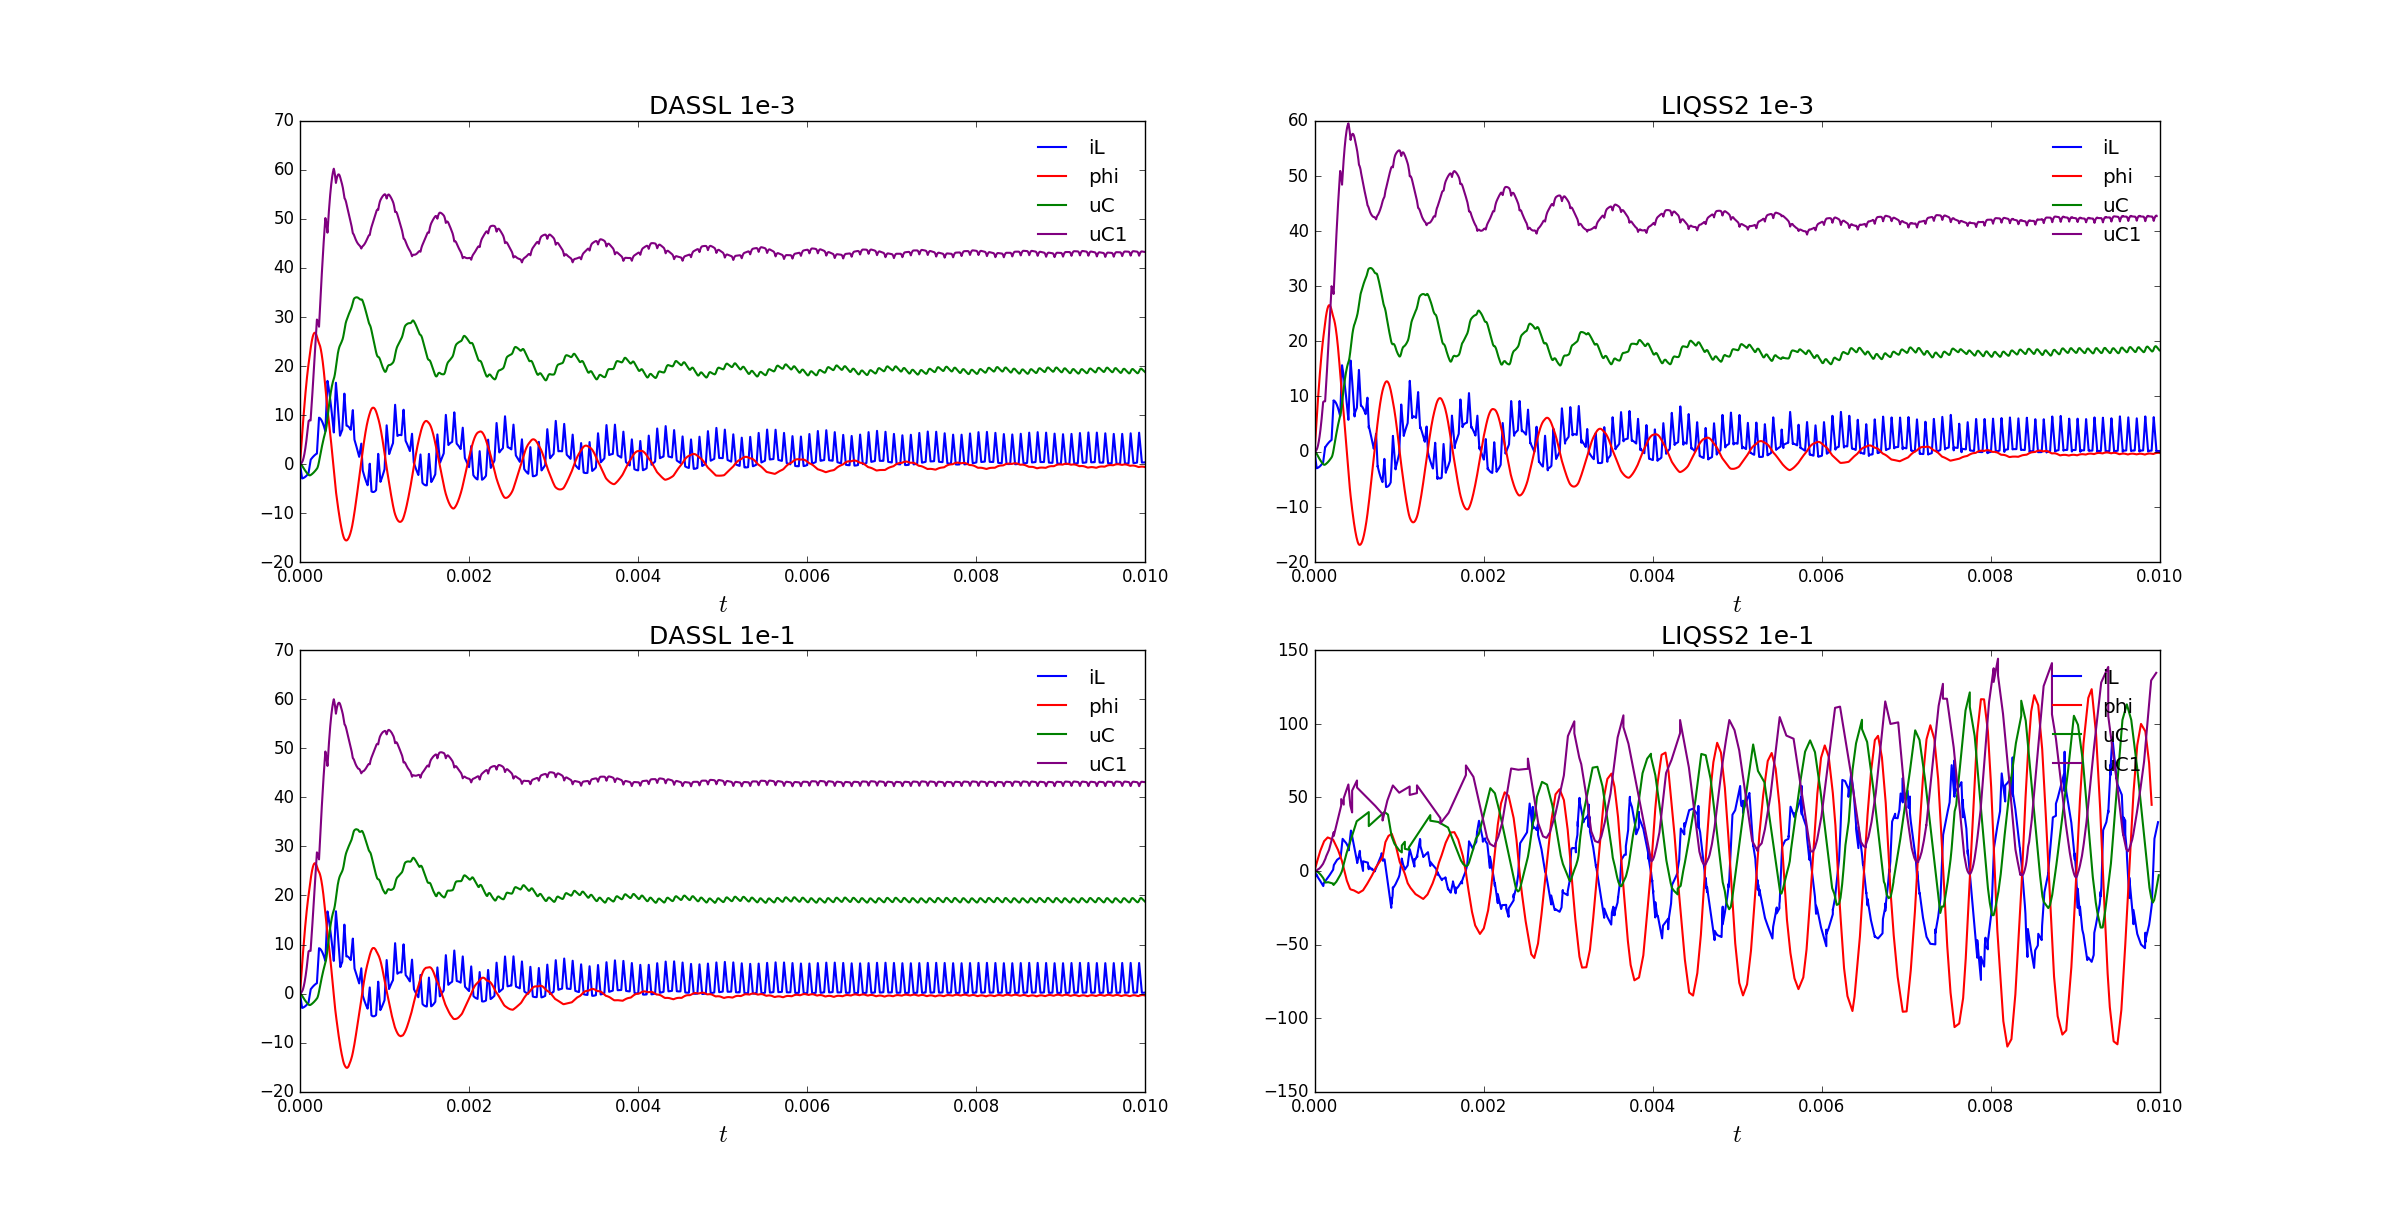
\includegraphics[scale=0.32, clip,trim={50mm 1mm 45mm 10mm}]{./Fig/Converter.png}
\vspace{-0.8cm}
\caption{Simulation results of the Buck Converter.}\label{Fig1}
\end{figure}

Figure~\ref{Fig1} displays the various simulation results for the Buck Converter model. The solvers and tolerances used are displayed in the captions of each subgraph. The LIQSS2 solver is very sensitive to values of the tolerances. If the tolerances are not restrictive, the simulations results are completely inaccurate, while if the tolerances are too restrictive the simulation times become unnecessarily excessive.

\newpage

\subsection{Bouncing ball}

The bouncing ball is an example of a hybrid system, containing events and conditional expressions. This model was simulated for 25 seconds in total. The simulation times are shown in Table~\ref{Tab2}. The tolerances has a great impact on the simulation results for the LIQSS2 solver. The simulation results are completely inaccurate for tolerances lower than {\tt{1e-6}}. The simulation results only improve for restrictive tolerances. The additional problem arises that the LifeQ LIQSS2 solver does not contain the {\sf{SC\_Update()}} function that is present in QSS Solver~\cite{qss}. This function, in QSS Solver, enables the LIQSS2 solver to accurately simulate the bouncing ball at less restrictive tolerances. The {\sf{SC\_Update()}} function contributes to the solver especially during the actual bouncing of the ball. Without this function the tolerances have to make up for the lack of implementation detail at the cost of incurring additional calculations and simulation time.

\begin{table}[htbp]
	\centering\footnotesize
		\begin{tabular}{ccc}
    \topline	\headcol
    Tolerance&{\sf DASSL}& {\sf LIQSS2}\\\midline
{\tt{1e-1}}&	0.067&	0.016\\\rowcol
{\tt{1e-2}}&	0.072&	0.007\\
{\tt{1e-3}}&	0.076&	0.011\\\rowcol
{\tt{1e-6}}&	0.077&	0.618\\
{\tt{1e-8}}&	0.083&	34.553\\\bottomline
    \end{tabular}
\caption{Simulation results of the Bouncing Ball.}
\label{Tab2}
    \end{table}

Figure~\ref{Fig2} shows the results of the simulations. DASSL is able to accurately simulate the bouncing ball model for less restrictive tolerances, while this is not possible the LIQSS2 solver. The LIQSS2 solver's most notable shortcoming is that the bouncing of the ball is erratic when the tolerances are relaxed. DASSL only loses less notable accuracy when the tolerance restrictions are relaxed.

    \begin{figure}[htbp]\centering
   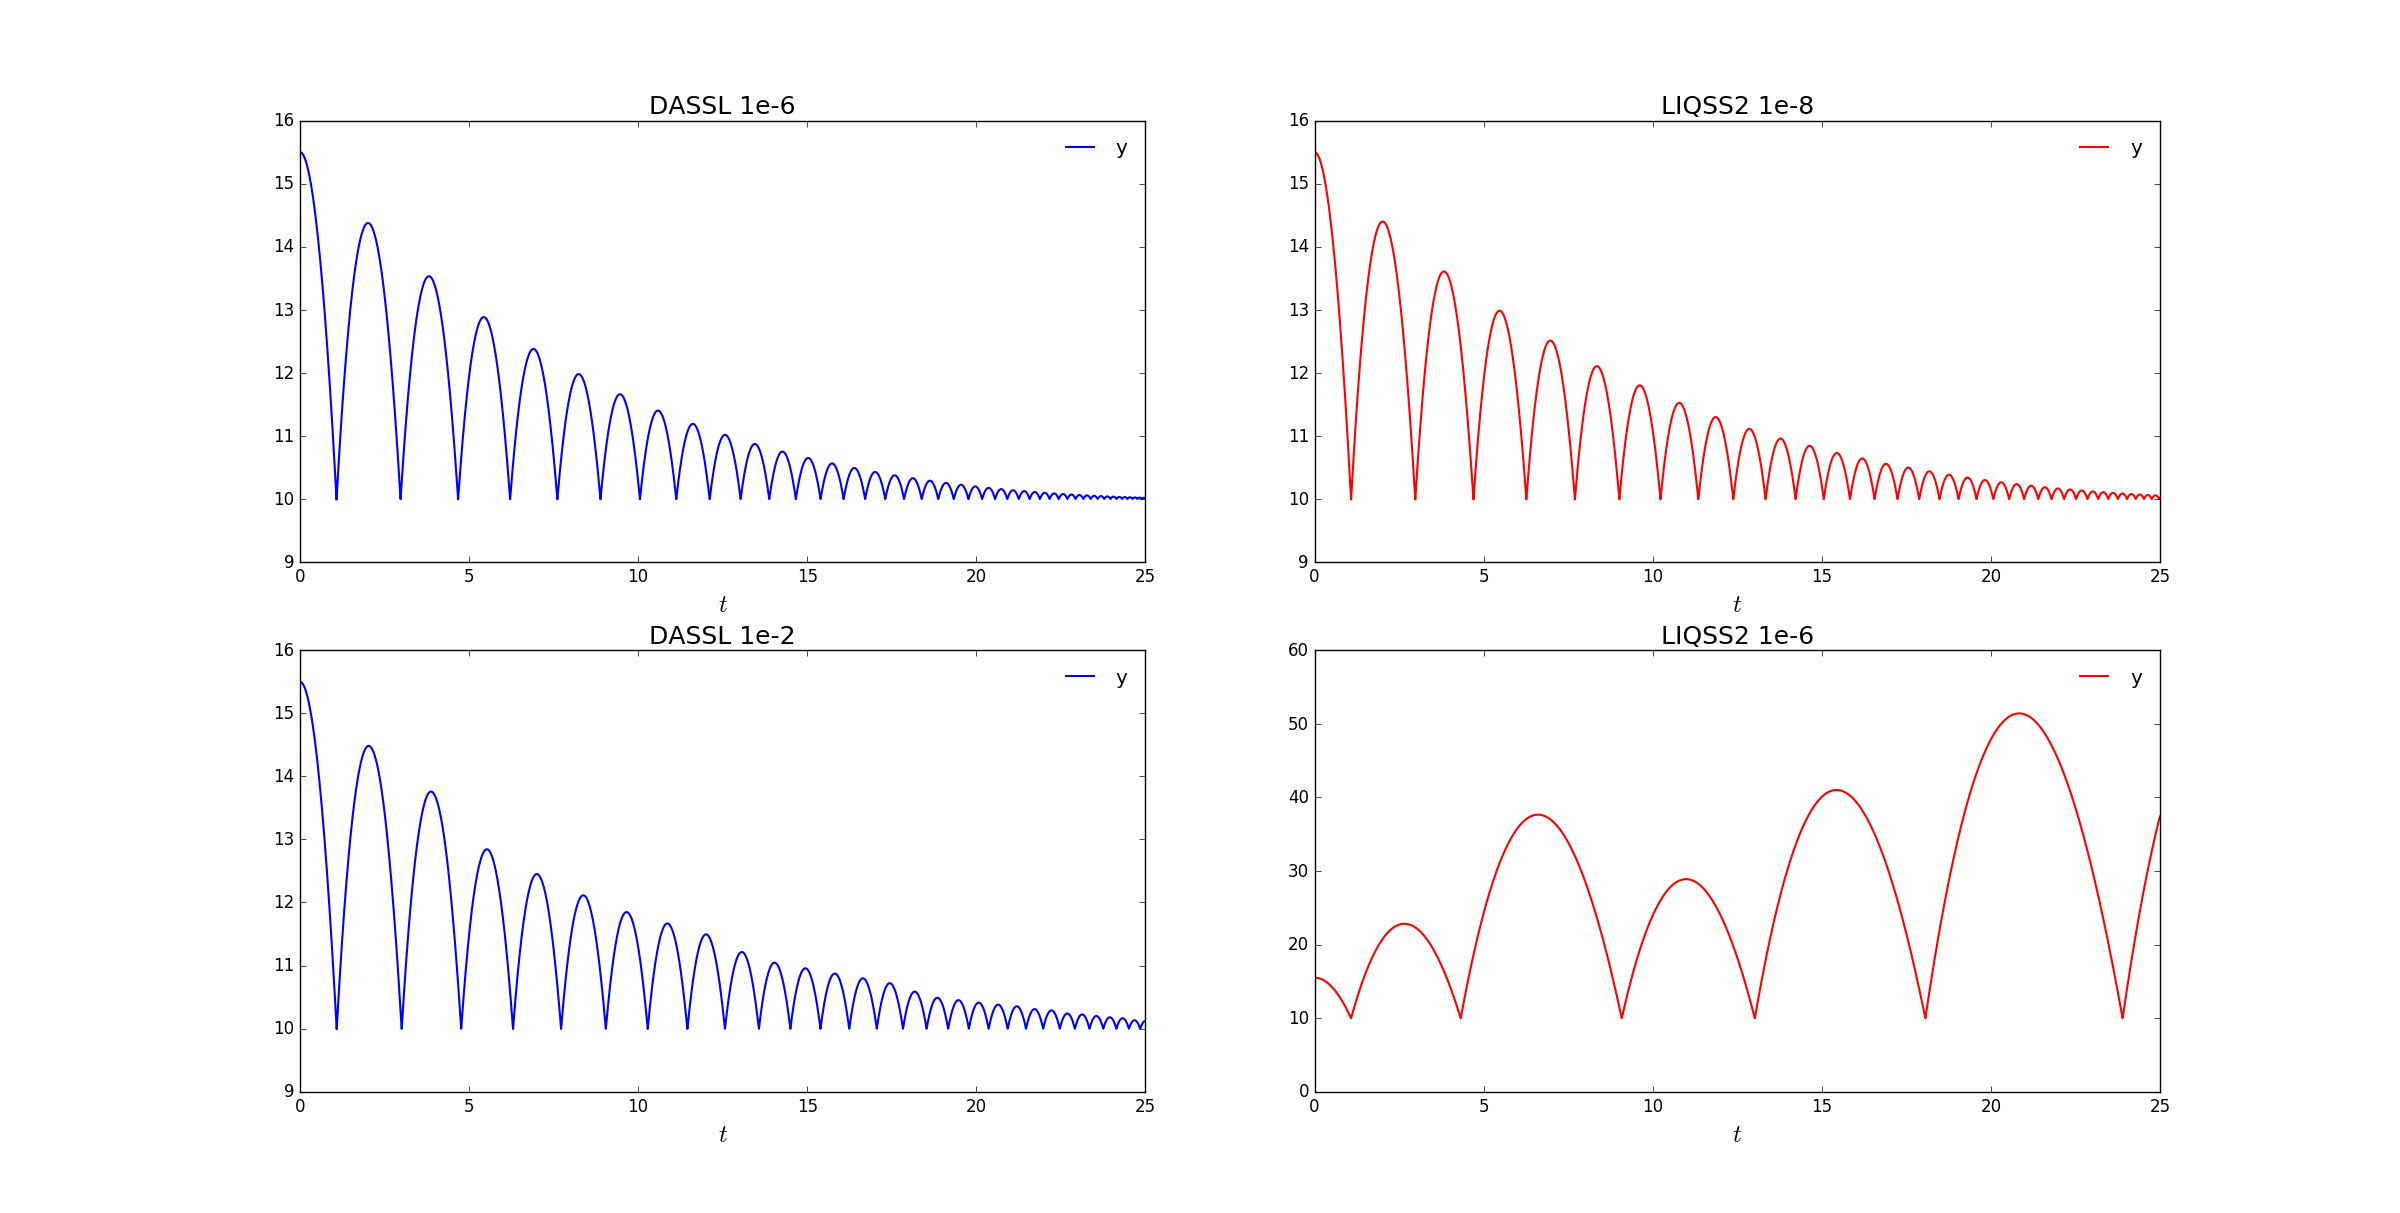
\includegraphics[scale=0.32, clip,trim={50mm 1mm 45mm 10mm}]{./Fig/BBall.png}
\vspace{-0.8cm}
\caption{Simulation results of the Bouncing Ball.}\label{Fig2}
\end{figure}

Although the LifeQ LIQSS2 solver can successfully simulate the bouncing ball problem, it is far from ideal and lacking in practical value.

\newpage
\subsection{Lotka-Volterra model}

The Lotka-Volterra model is a simple model to simulate and can be simulated for varying periods of time as the oscillations should repeat identically as the simulation time progresses. Table~\ref{Tab3} shows the simulation times for the Lotka-Volterra model for 40 seconds and 4\,000 seconds, respectively. The simulation times are relatively consistent between the various tolerances for the DASSL solver. Again, it is clear that the tolerances have a significant impact on the simulation times of the LIQSS2 solver.



\begin{table}[htbp]

    \begin{minipage}{.5\linewidth}
      \centering
		\begin{tabular}{ccc}
    \topline	\headcol
    Tolerance&{\sf DASSL}& {\sf LIQSS2}\\\midline
{\tt{1e-2}}&	0.063&	0.028\\\rowcol
{\tt{1e-3}}&	0.063&	0.071\\
{\tt{1e-5}}&	0.064&	2.523\\\rowcol
{\tt{1e-8}}&	0.066&	29.485\\\bottomlinec
    \end{tabular}
       \newline \newline (a) Total simulation time = 40 seconds
    \end{minipage}%
    \begin{minipage}{.5\linewidth}
      \centering
		\begin{tabular}{ccc}
    \topline	\headcol
    Tolerance&{\sf DASSL}& {\sf LIQSS2}\\\midline
{\tt{1e-2}}&	0.088&	0.896\\\rowcol
{\tt{1e-3}}&	0.103&	2.847\\
{\tt{1e-5}}&	0.164&	339.513\\\rowcol
{\tt{1e-8}}&	0.285&	Seg fault\\\bottomlinec

    \end{tabular}
    \newline \newline (b) Total simulation time = 4\,000 seconds
    \end{minipage}
    \caption{Simulation results of Lotka-Volterra.}
    \label{Tab3}
\end{table}


The numerical results of the  Lotka-Volterra model simulated for 40 seconds are shown in Figure~\ref{Fig3}. For non-restrictive tolerances the oscillations systematically deviate from the expected behaviour. The amplitude of the oscillation become smaller, which is a draw-back when simulating with non-restrictive tolerances. This problem occurs in both solvers, but is more prevalent in the LIQSS2 solver.

    \begin{figure}[htbp]\centering
   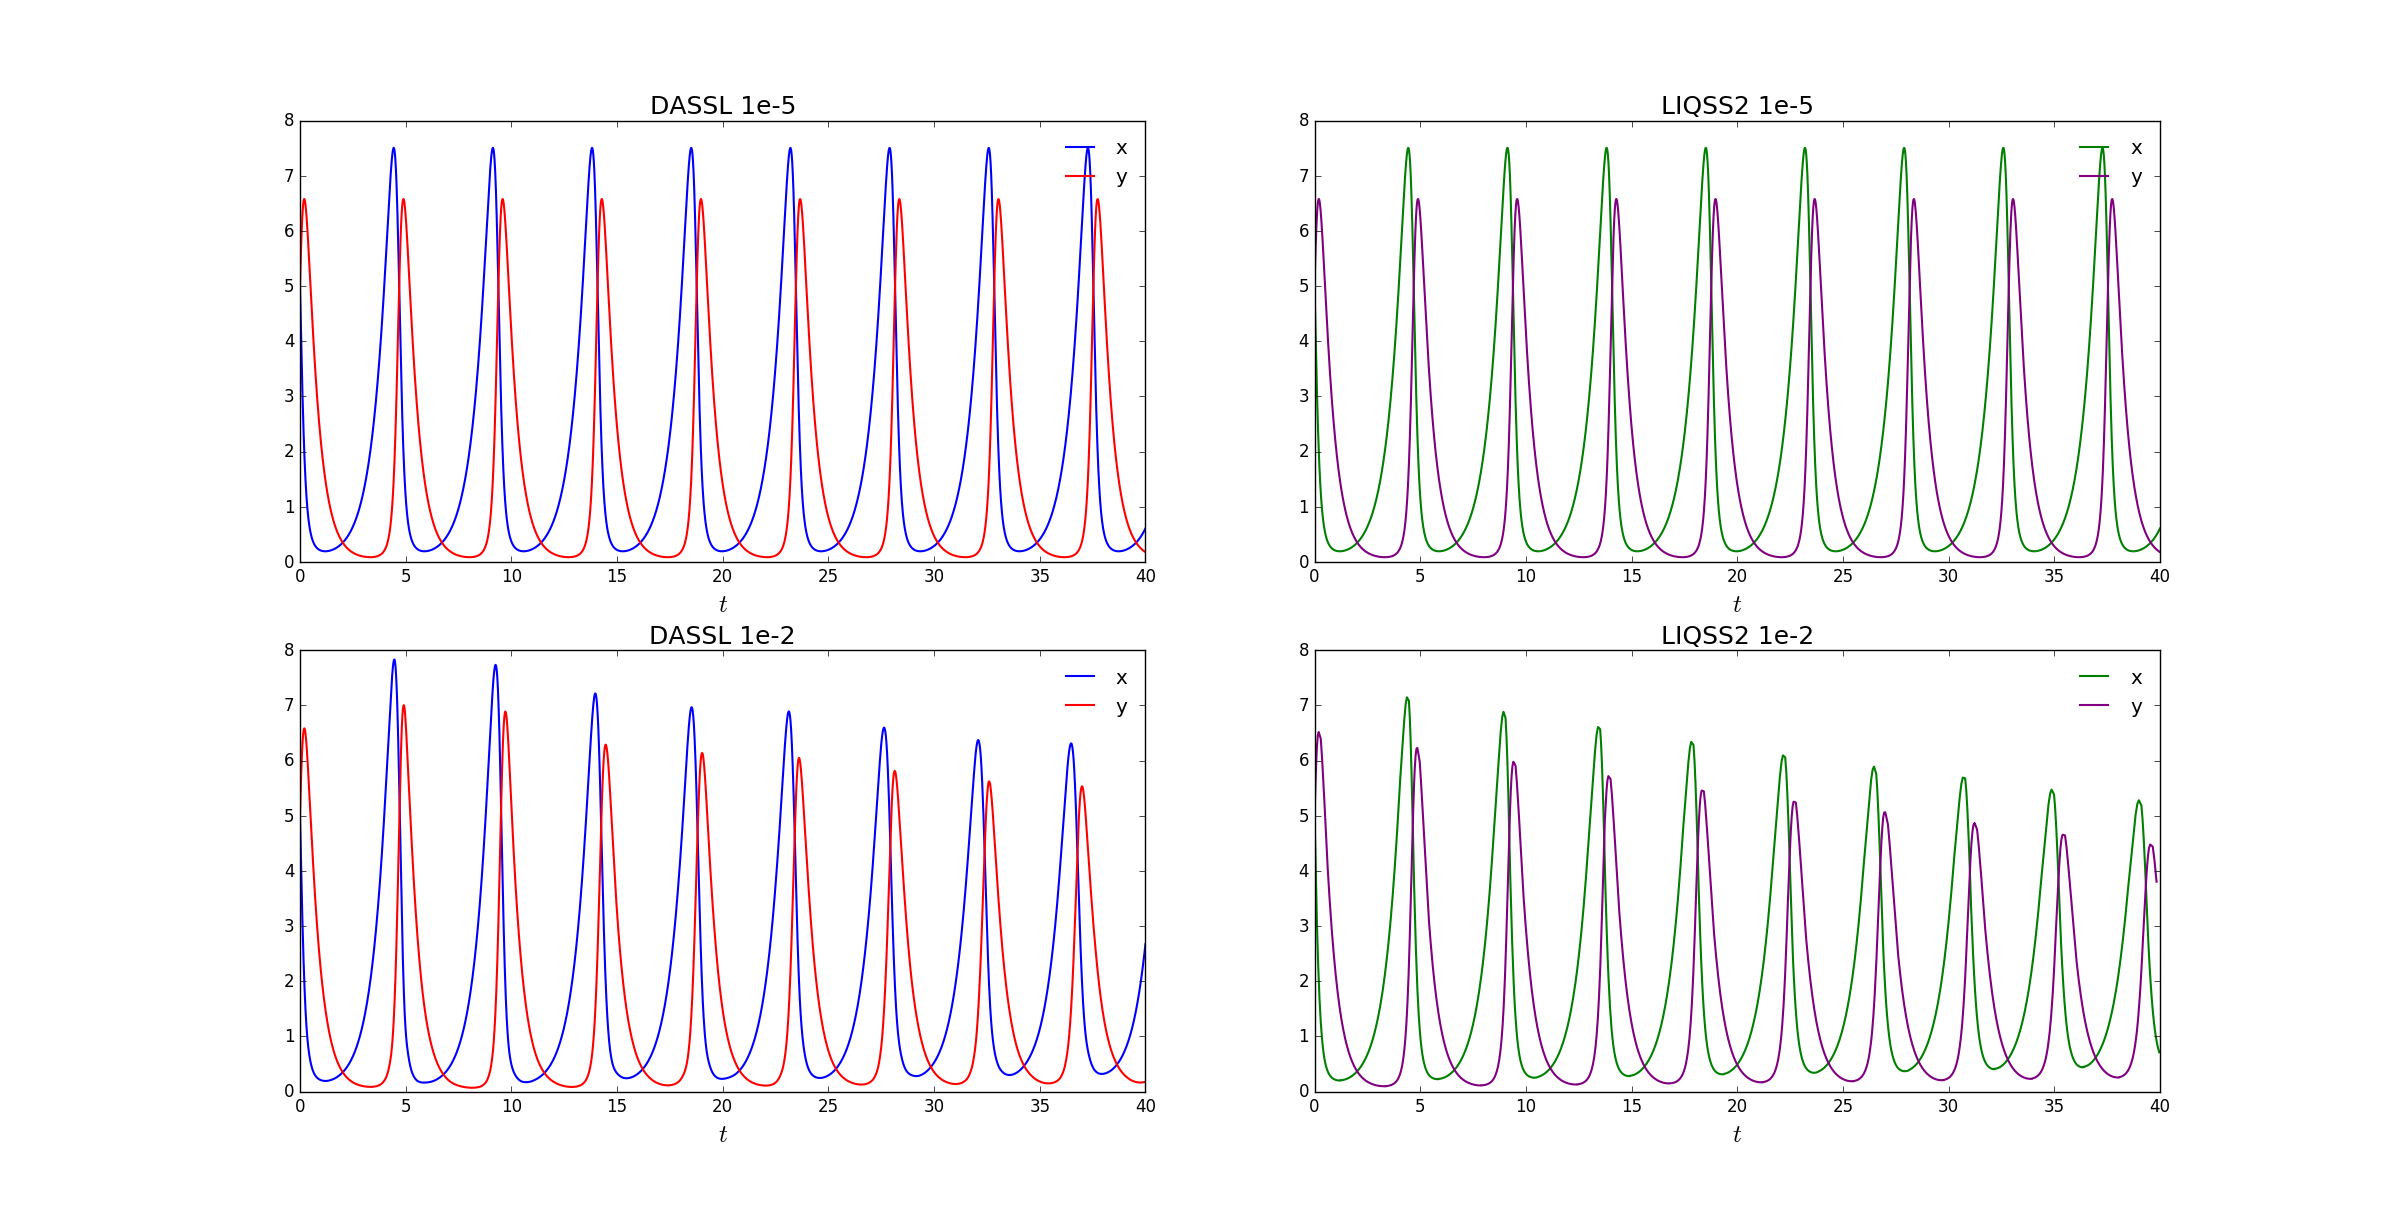
\includegraphics[scale=0.32, clip,trim={50mm 1mm 45mm 10mm}]{./Fig/LV.png}
\vspace{-0.8cm}
\caption{Simulation results of the Lotka-Volterra model.}\label{Fig3}
\end{figure}

It is important to note that the simulation times do not increase dramatically when the stoptime of the simulations are increase for the DASSL solver. This is in contrast to the LIQSS2 solver for which the total simulation times increase substantially when the simulation stopTimes are increased (from 40 seconds to 4\,000 seconds).

\newpage

\subsection{Van der Pol Oscillator}

The Van der Poll oscillator is system consisting of two state variables. The mathematical stiffness of this model can be increased by altering a single variable of the model. The model contains a parameter $\lambda$ which is correlated to the mathematical stiffness of the model. Results are shown for $\lambda=1$ where the simulation time is specified as 50 seconds. An experiment which is deemed as ``more'' stiff is where $\lambda=30$ and these models are simulated for 500 seconds in total.

\begin{table}[htbp]

    \begin{minipage}{.5\linewidth}
      \centering
		\begin{tabular}{ccc}
    \topline	\headcol
    Tolerance&{\sf DASSL}& {\sf LIQSS2}\\\midline
{\tt{1e-2}}&	0.052&	0.039\\\rowcol
{\tt{1e-3}}&	0.054&	0.109\\
{\tt{1e-5}}&	0.079&	0.915\\\rowcol
{\tt{1e-8}}&	0.094&	---
\\\bottomlinec
    \end{tabular}
       \newline \newline (a) Total simulation time = 50 seconds, $\lambda = 1$
    \end{minipage}%
    \begin{minipage}{.5\linewidth}
      \centering
		\begin{tabular}{ccc}
    \topline	\headcol
    Tolerance&{\sf DASSL}& {\sf LIQSS2}\\\midline
{\tt{1e-2}}&	0.052&	1.48\\\rowcol
{\tt{1e-3}}&	0.052&	4.246\\
{\tt{1e-5}}&	0.056&	36.196\\\rowcol
{\tt{1e-8}}&	0.061&	---\\\bottomlinec

    \end{tabular}
    \newline \newline (b) Total simulation time = 500 seconds, $\lambda = 30$
    \end{minipage}
    \caption{Simulation results of Van der Pol oscillator.}
    \label{Tab4}
\end{table}


The numerical results of the Van der Pol oscillator are shown in Figure~\ref{Fig4}. The two solvers provide similar results for the two models. The LIQSS2 solver is able to find the exact turning points of the variable $y$. The simulation times differs between the solvers when the tolerances are made more restrictive.

    \begin{figure}[htbp]\centering
   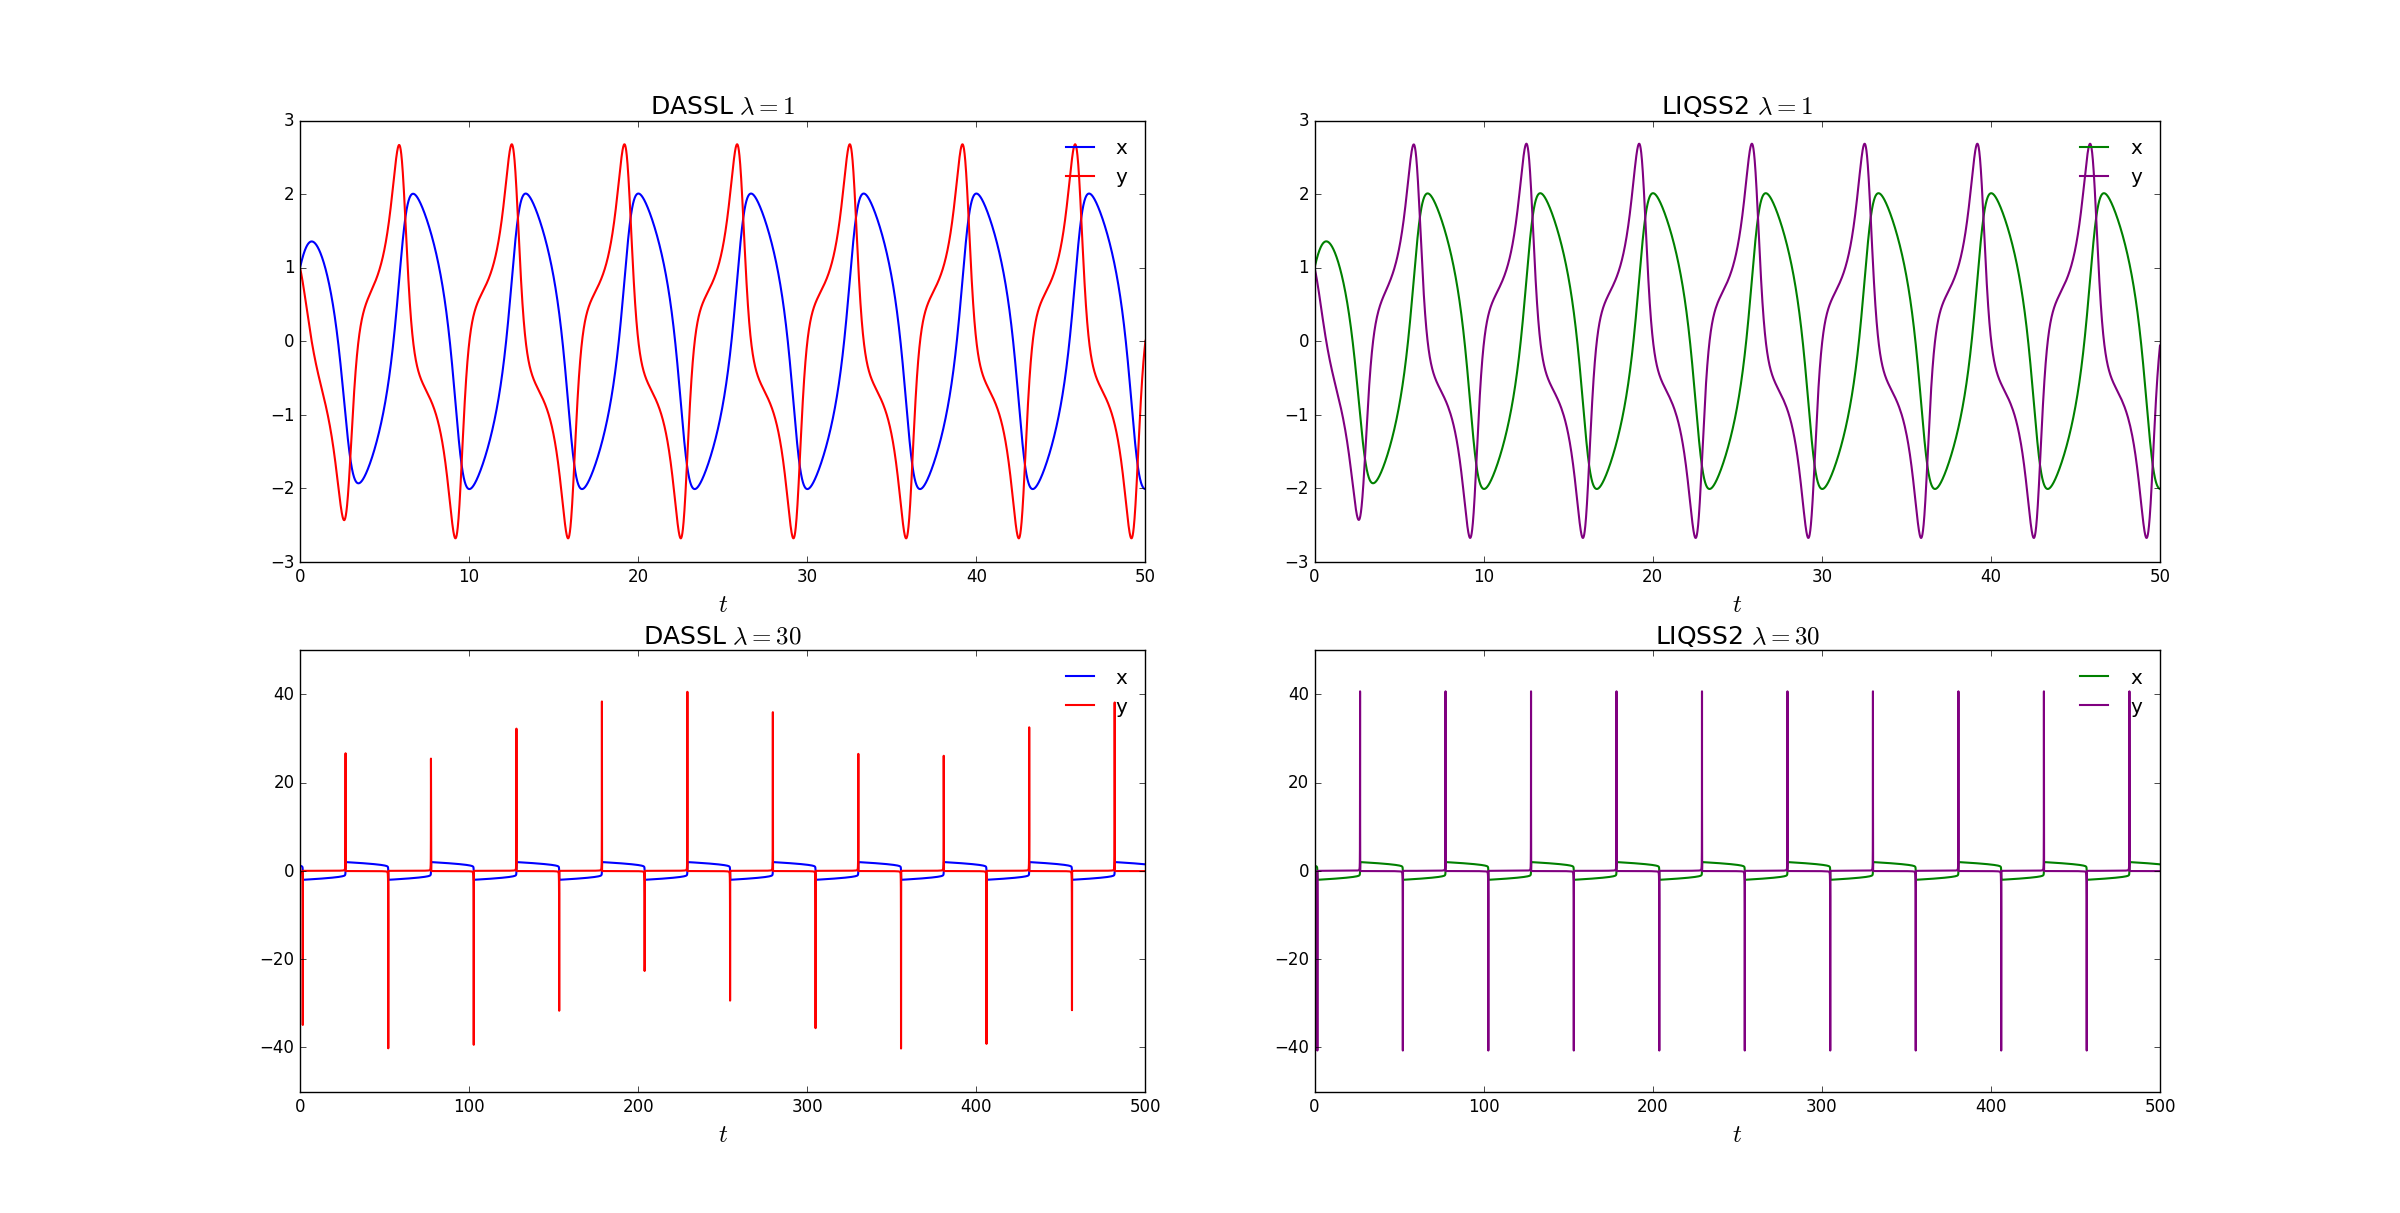
\includegraphics[scale=0.32, clip,trim={50mm 1mm 45mm 10mm}]{./Fig/VDP.png}
\vspace{-0.8cm}
\caption{Simulation results of the Van der Pol oscillator.}\label{Fig4}
\end{figure}

The Van der Pol oscillator demonstrates that the LIQSS2 solver can simulate stiff mathematical models. The DASSL solver, however, is also capable of simulating the model accurately.

\newpage

\subsection{Advection-reaction model}

This example is the {\em method of line discretization} of an advection–reaction model. This model contains 900 state variables and is thus used to showcase LifeQ's LIQSS2 solver when solving a stiff mathematical system containing a large number of state variables. The model is simulated for 1 second. The simulation times for the various tolerances used is showed in Table~\ref{Tab5}.

\begin{table}[htbp]
	\centering\footnotesize
		\begin{tabular}{ccc}
    \topline	\headcol
    Tolerance&{\sf DASSL}& {\sf LIQSS2}\\\midline
{\tt{1e-2}}&	6.872&	49.02\\\rowcol
{\tt{1e-3}}&	7.302&	105.152\\
{\tt{1e-6}}&	8.812&	---\\\rowcol
{\tt{1e-8}}&	11.292&	---\\\bottomlinec
    \end{tabular}
\caption{Simulation results of the advection-reaction model.}
\label{Tab5}
    \end{table}

Notice that the simulation times of the LifeQ LIQSS2 solver far exceeds that of the DASSL solver. The simulation times of the LIQSS2 solver of QSS Solver are however much faster than both the DASSL solver and LifeQ LIQSS2 solver. This may be attributed to the additional elements in the QSS Solver framework that is lacking in the LifeQ LIQSS2 solver.

Figure~\ref{Fig5} shows the numerical results of the simulations for this model. Both solvers used can simulate the model accurately. Small numerical errors are incurred when the tolerances are relaxed in the LifeQ LIQSS2 solver.

    \begin{figure}[htbp]\centering
   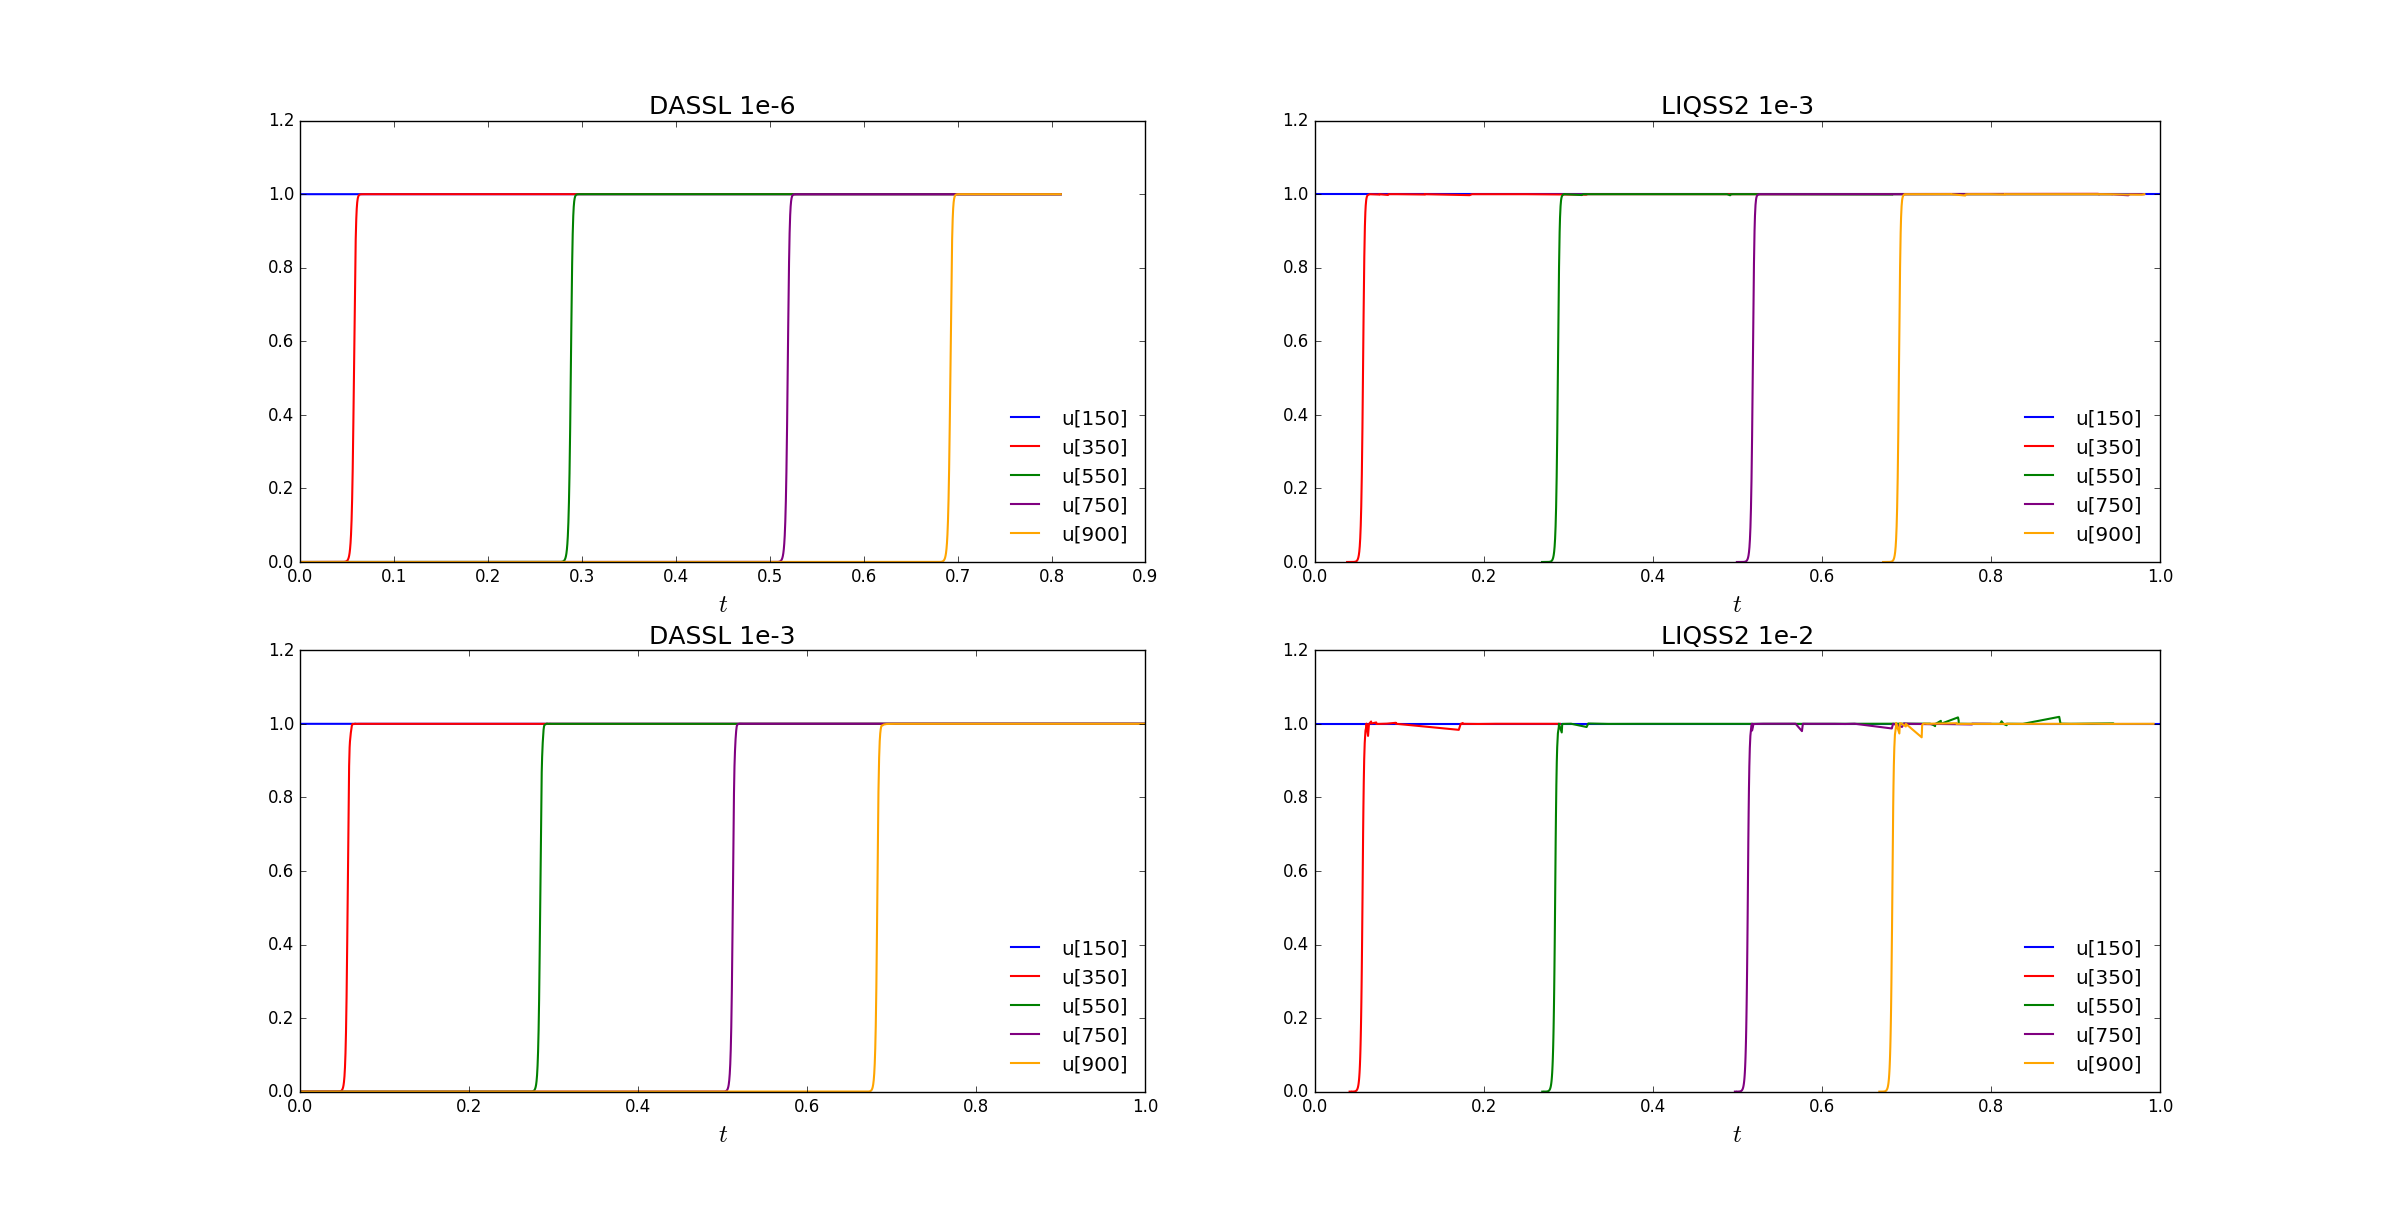
\includegraphics[scale=0.32, clip,trim={50mm 1mm 45mm 10mm}]{./Fig/advection.png}
\vspace{-0.8cm}
\caption{Simulation results of the advection-reaction model.}\label{Fig5}
\end{figure}

This demonstrates that the LifeQ LIQSS2 solver is able to simulate models containing a large number of state variables in a stiff mathematical system.

\newpage

\subsection{Danielsen Ottesen model}

No successful simulation of the Danielsen Ottesen model has been performed with the LIQSS2 solver. From LifeQ's perspective there should not be any reason why the model cannot be simulated by this solver. There may be inefficiencies within the model, but this should not influence the simulation results in the current manner that is does. At this stage model executions are halted since OpenModelica reports errors realted to the non-linear solvers when attempting to simulate the model. This problem is incurred after only a fraction of one simulation second. Therefore no meaningful results have yet been obtained for the Danielsen Ottesen model.

From this point there are two approaches that LifeQ can use to find progress in this matter. The first option is to investigate the reason for the failure of the non-linear solvers within OpenModelica, which may take a substantial amount of time. The alternative option is to reduce the Danielsen Ottensen model ({\em e.g.}\ by removing valves and other components) until a model is found that can be simulated. The model can then be appended iteratively until a working model is found.

Figure~\ref{Fig6} shows the numerical results of the Danielsen Ottesen model for the DASSL solver and the LifeQ LIQSS2 solver. Although the LifeQ LIQSS2 solver does not simulate the two variables correctly, the patterns do repeat in conjunction with the timing of the changes in results of the DASSL solver.

    \begin{figure}[htbp]\centering
   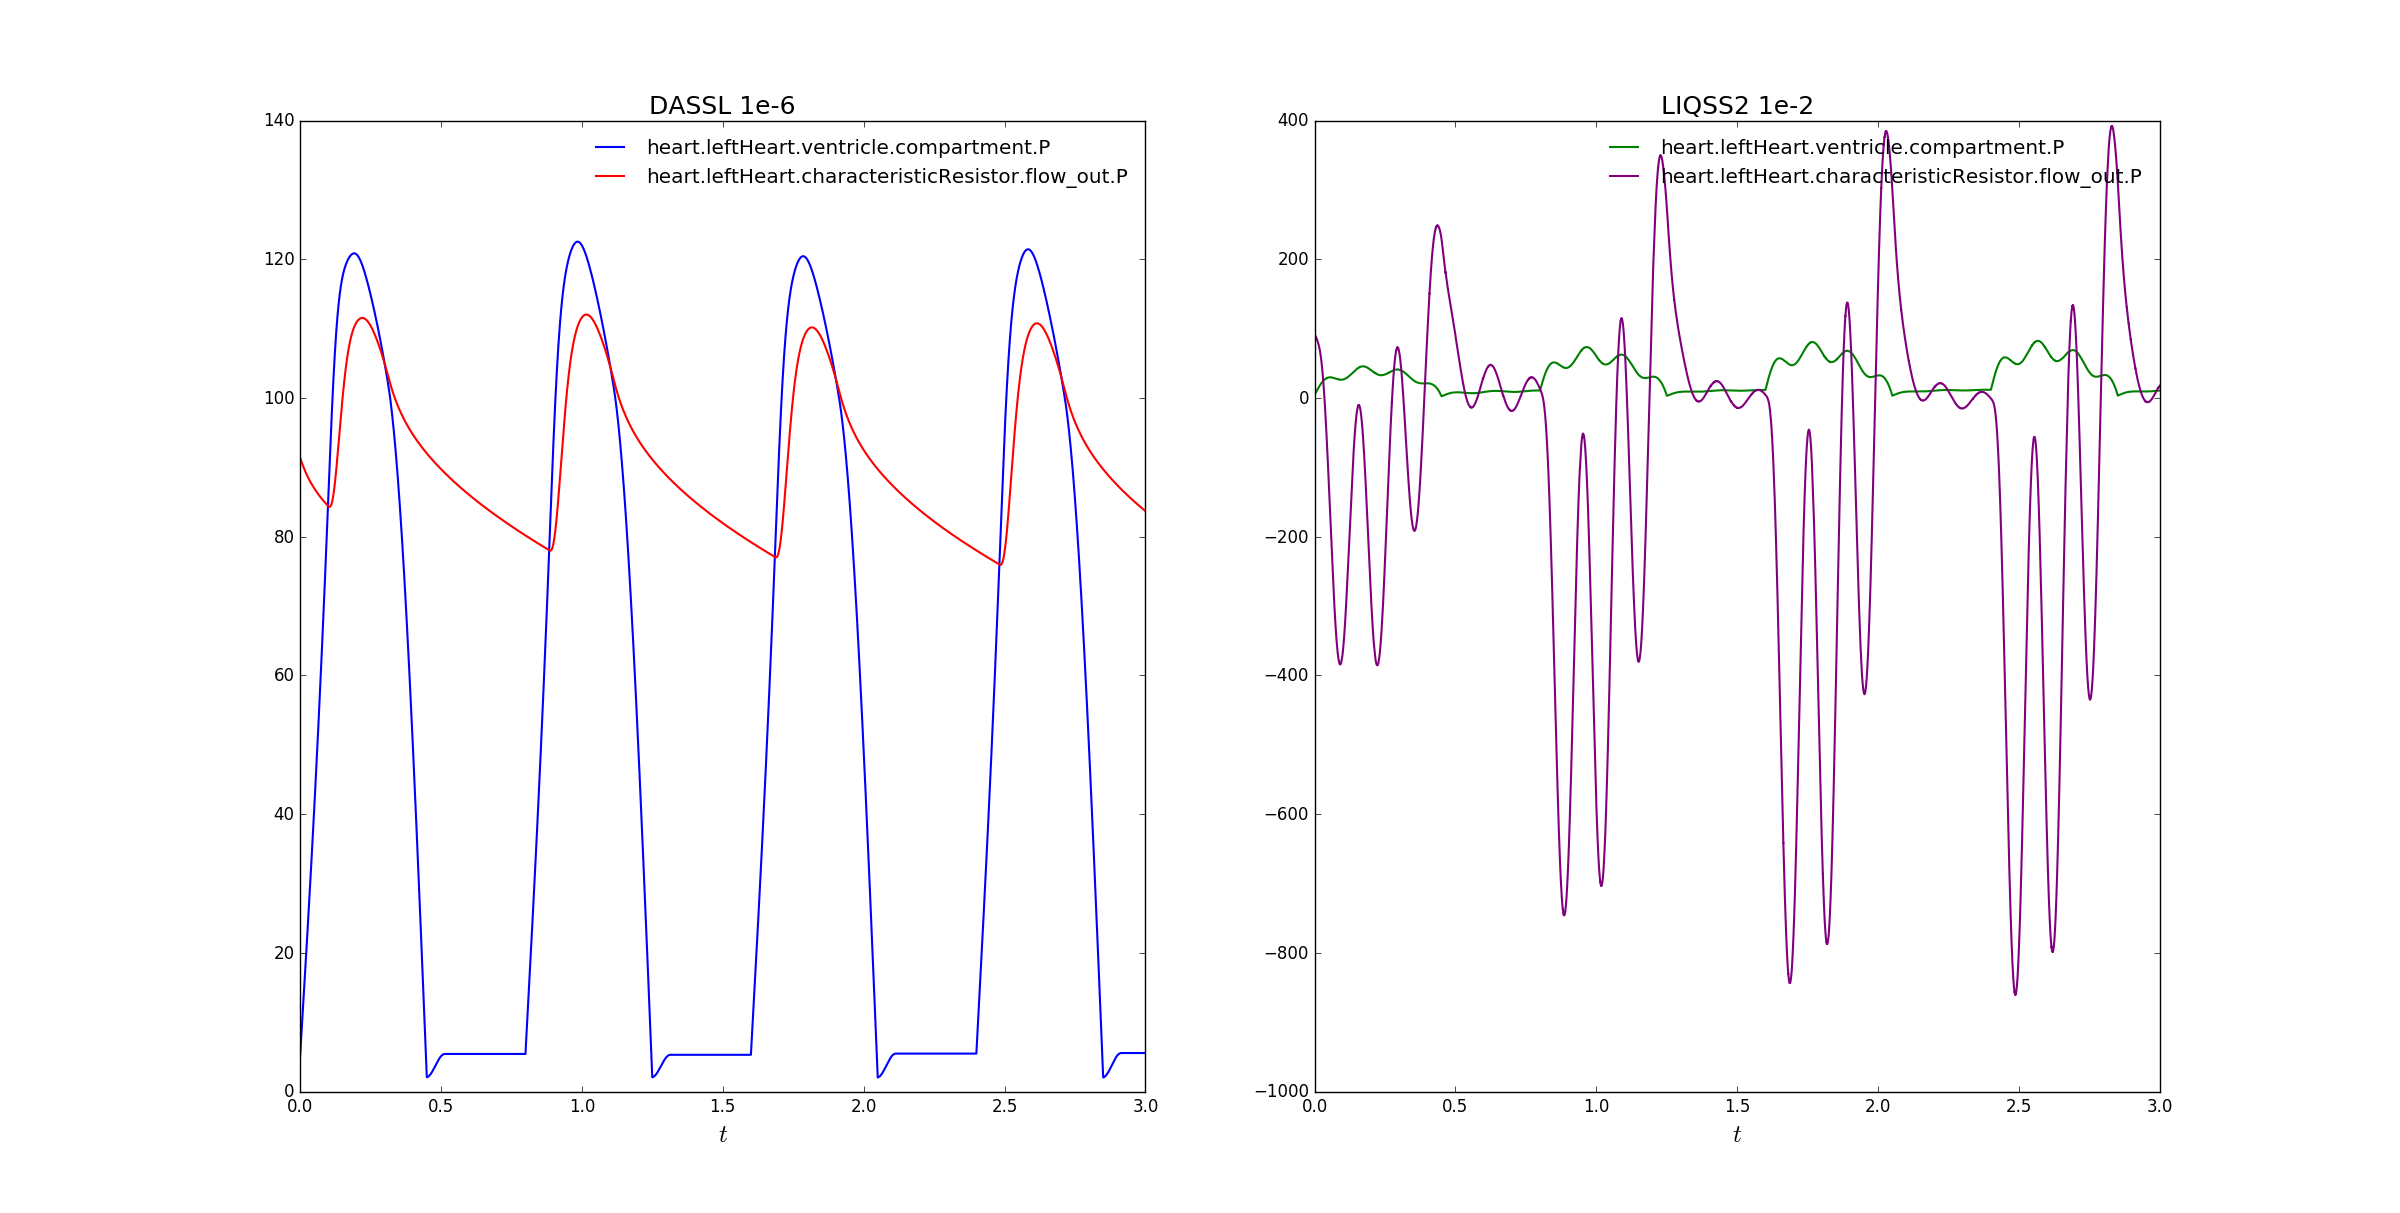
\includegraphics[scale=0.32, clip,trim={50mm 1mm 45mm 10mm}]{./Fig/Daniel.png}
\vspace{-0.8cm}
\caption{Simulation results of the Danielsen Ottesen model.}\label{Fig6}
\end{figure}

These results are promising in the sense that sections (groups) of oscillations do repeat as expected at the expected time steps during the simulation.

\newpage

\section{Conclusions and future work}

The results in this document show promising results for the LifeQ LIQSS2 solver. Although this solver is not yet able to simulate the Danielsen Ottesen model, it does display the required elements to suggest that it should be capable of solving the model. The tolerances have a significant impact on the simulation times and accuracy of models solved by the LIQSS2 solver.

There are known shortcomings of the LifeQ LIQSS2 solver, which should be addressed to ensure that the solver is capable of simulating any model in general. Furthermore, collaboration from the authors of QSS Solver should enable LifeQ to fast-track the process of refining the LifeQ LIQSS2 solver. Interaction with the developers of OpenModelica may also aid in implementing the solver in the correct and most efficient manner.


{\footnotesize
\begin{thebibliography}{10}

\bibitem{qss2}{\sc Fern\'andez J \& Kofman E}, 2014, {\em A stand-alone quantized state system solver for continuous system simulation}, Simulation, {\bf{90(7)}}, pp.\, 782--779.


\bibitem{OMCompiler} {\sc OMCompiler}, 2016, {\em LifeQ OMCompiler submodule repository}, [Online], Cited 15\textsuperscript{th} March 2016, Available from {\url{https://bitbucket.org/antonpdv/omcompiler}}

\bibitem{OpenModelica} {\sc OpenModelica}, 2016, {\em Open Source Modelica Consortium}, [Online], Cited 15\textsuperscript{th} March 2016, Available from {\url{https://openmodelica.org/}}

\bibitem{DASSL}{\sc Petzold LR}, 1982, {\em A description of DASSL: A differential/algebraic system solver}, Technical Report, Applied Mathematics Division, Sandia National Laboratories, Livermore (CA).

\bibitem{qss}{\sc QSS Solver}, 2016, {\em Modeling and simulation tool for continuous and hybrid systems}, [Online], Cited 15\textsuperscript{th} March 2016, Available from {\url{https://sourceforge.net/projects/qssengine/}}


\end{thebibliography}}


\end{document}